\documentclass{article} % For LaTeX2e
\usepackage{iclr2018_conference,times}
\usepackage{hyperref}
\usepackage{url}
\usepackage{graphicx}
%% To use subfigures
\usepackage{subcaption}
%% To place figures where you want to
\usepackage{float}
%% To remove whitespace before enumerate
\usepackage{enumitem}
%% For thicker table horizontal lines
\usepackage{booktabs}

\title{Deep Sentiment Analysis on Tumblr}

% Authors must not appear in the submitted version. They should be hidden
% as long as the \iclrfinalcopy macro remains commented out below.
% Non-anonymous submissions will be rejected without review.

\author{Anthony Hu \& Seth Flaxman \\
Department of Statistics\\
University of Oxford\\
Oxford, United Kingdom \\
\texttt{\{anthony.hu,flaxman\}@stats.ox.ac.uk}
}

% The \author macro works with any number of authors. There are two commands
% used to separate the names and addresses of multiple authors: \And and \AND.
%
% Using \And between authors leaves it to \LaTeX{} to determine where to break
% the lines. Using \AND forces a linebreak at that point. So, if \LaTeX{}
% puts 3 of 4 authors names on the first line, and the last on the second
% line, try using \AND instead of \And before the third author name.

\newcommand{\fix}{\marginpar{FIX}}
\newcommand{\new}{\marginpar{NEW}}

%\iclrfinalcopy % Uncomment for camera-ready version, but NOT for submission.

\begin{document}


\maketitle

\begin{abstract}
We introduce a new large-scale multimodal dataset for sentiment analysis named TumblrData, that contains over 1 million labeled data with text, image and the associated emotion, as a new mean of evaluation of machine learning models using visual and textual contents for sentiment analysis research.

We propose a novel approach to sentiment analysis using deep neural networks combining visual recognition and natural language processing. Our approach leverages Tumblr posts containing images and text to predict the emotional state of users. Deep convolutional layers extract relevant features from images and high-dimensional word embedding followed by a recurrent layer process the textual information in order to infer the emotion conveyed by a given Tumblr post. We demonstrate that our network architecture, named Deep Sentiment, learns meaningful relations between visual data and language as it outperforms models using a single modality.% We then show that Deep Sentiment can also be adapted to generate images and text representative of an emotion. 
\end{abstract}

\section{Introduction}
Sentiment analysis has been an active area of research in the past few years, especially on the readily available Twitter data, e.g. \citet{Bollen} who investigated the impact of collective mood states on stock market or \cite{Flaxman-16} who analysed day-of-week population well-being.

Contrary to Twitter, Tumblr posts are not limited to 140 characters, allowing more expressiveness, and are not focused on the textual content but on the visual content. A Tumblr post will almost always be an image with some text accompanying the latter. Pictures have become prevalent on social media and characterising them could enable the understanding of billions of users. Unfortunately, there is no large publicly available dataset for multimodal sentiment analysis. This paper provides a new dataset, TumblrData \footnote{\texttt{https://github.com/anthonyhu/tumblr-sentiment}}, that will allow the research community to learn multimodal feature representations of emotions.

Also, we propose a novel method to uncover the emotional state of an individual posting on social media. The ground truth emotion will be extracted from the Tumblr tags, considered as the `self-reported' emotion of the user. Our model incorporates both text and image and we aim to `read' them to be able to understand the emotional content they imply about the user. Concretely, the Deep Sentiment model associates the features learned by the two modalities as follows:

\begin{itemize}
    \item We fine-tune a pre-trained deep convolutional neural network, named Inception \citep{Szegedy-15}, to our specific task of emotion inferring.
    \item We project the text in a rich high-dimensional space with a word representation learned by GloVe \citep{Pennington-14} The word vectors then go through a recurrent neural network which preserves the word order and captures the semantics of human language.
    \item A fully-connected layer combines the information in the two modalities and a final softmax output layer gives the probability distribution of the emotional state of the user.
\end{itemize}

%We will also see that Deep Sentiment can be rearranged to generate Tumblr posts expressing one of the learned emotion.

\section{TumblrData}

Tumblr is a microblogging service where users post multimedia content with the following attributes: an image, text and tags. The tags are really valuable as they indicate the user's state of mind when writing his post. 

To build our dataset, queries were made through the Tumblr API searching for an emotion appearing in the tags. The 16 emotions retained are those with a high relative frequencies among the PANAS-X scale \citep{PANAS-X}. In some posts, the tag containing the emotion of the post also appeared in the text itself, undermining the possibility of learning meaningful relationships between the features and the emotion expressed. We thus removed from the text the tags containing the emotion to be predicted.

Tumblr is used worldwide but we only kept posts written in English. Basically, if a post contained less than a given number of English word, it was deemed as non-English and removed from the dataset. The threshold was set to 5 English words as it appeared to filter out reasonably well non-English posts. [To change: filter posts with less than 90\% of English words] The vocabulary of English words was obtained from GloVe. Figure \ref{fig:emotions} shows two posts with their associated emotions and table \ref{tumblrdata} summarises the statistics of the data.

\begin{figure}[H]
    \begin{subfigure}[t]{.5\textwidth}
        \vskip 0pt %Necessary to align on image and not caption
        \centering
        
\includegraphics[width=.2\linewidth]{Images/optimistic.jpg}
        \caption{\textbf{Optimistic}: ``The most beautiful thing we can experience is the mysterious. It is the source of all true art and science -- Albert Einstein."}
   \end{subfigure}
   \begin{subfigure}[t]{.5\textwidth}
       \vskip 0pt
       \centering
       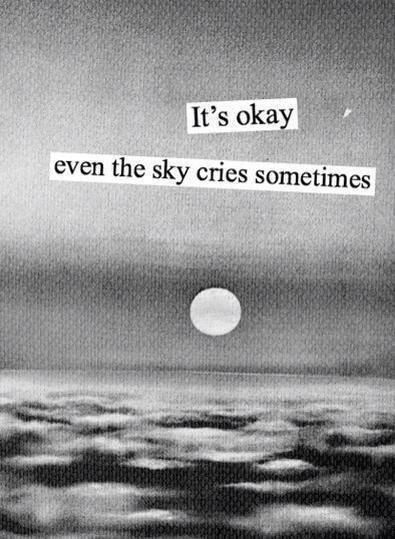
\includegraphics[width=.2\linewidth]{Images/sad.jpg}
       \caption{\textbf{Sad}: ``It's okay to be upset. It's okay to not always be happy. It's okay to cry. Never hide your emotions in fear of upsetting others or of being a bother."}
    \end{subfigure}
    \caption{Examples of Tumblr posts}
    \label{fig:emotions}
\end{figure}

\begin{table}[H]
\caption{Summary statistics for the TumblrData dataset, that spans from January 2011 to September 2017}
\begin{center}
    \begin{tabular}{ccc}
    \multicolumn{3}{c}{{\large \textbf{TumblrData}}} \\
    \addlinespace[0.2cm]
    \toprule
    Posts & In English & With Image \\
    \midrule
    1,015,140 & 582,231 & 258,803 \\
    \bottomrule
    \end{tabular}
	
    \vspace{0.2cm}
    
    \begin{tabular}{lrrr}
    \toprule
    Emotion & Posts & In English & With Image\\
    \midrule
Happy & 189,841 & 62\% & 29\% \\
Calm & 139,911 & 37\% & 29\% \\
Sad & 124,900 & 53\% & 15\% \\
Scared & 104,161 & 65\% & 20\% \\
Bored & 101,856 & 54\% & 29\% \\
Angry & 100,033 & 60\% & 21\% \\
Annoyed & 72,993 & 78\% & 10\% \\
Love & 66,146 & 61\% & 39\% \\
Excited & 37,240 & 58\% & 41\% \\
Surprised & 18,322 & 47\% & 32\% \\
Optimistic & 16,111 & 64\% & 36\% \\
Amazed & 10,367 & 61\% & 35\% \\
Ashamed & 10,066 & 63\% & 22\% \\
Disgusted & 9,178 & 69\% & 17\% \\
Pensive & 8,409 & 57\% & 34\% \\
Interested & 5,606 & 63\% & 32\% \\
    \bottomrule
    \end{tabular}
    
    %\vspace{0.2cm}
    
    %\begin{tabular}{ccc}
    %\toprule
    %\multicolumn{3}{c}{Text statistics (nb of words)} \\
    %\midrule
    %Min & Mean & Max \\
    %5 & 23 & 11310 \\
    %\bottomrule
    %\end{tabular}
\end{center}
\label{tumblrdata}
\end{table}

\section{Visual recognition}
Pictures are valuable to accurately infer the emotion expressed by a user. For instance, optimistic photos might contain vivid colors while sad pictures might contain darker colors. To extract visual insights from images, we will use convolutional neural networks, which achieve state-of-the-art performances in many visual recognition tasks.

\subsection{Transfer learning}
Training a convolutional network from scratch can be difficult as a large amount of data is needed and many different architectures need to be tested before achieving satisfying performances. To circumvent this issue, we can take advantage of the pre-trained network named Inception that learned to recognise images through the ImageNet dataset with a deep architecture of 22 layers.

Inception learned representations capturing the colors and arrangement of shapes of an image, which turn out to be relevant when dealing with images even for a different task. We could also say that the pre-trained network grasped the underlying structure of images. This statement rests on the hypothesis that all images lie in a low-dimensional manifold, and recent advances in realistic photos generation through generative adversarial networks bolsters this idea \citep{Radford-16}. 

More specifically, the Inception network learned to recognise features in a picture in order to classify the latter among the 1000 classes in the ImageNet dataset. Suppose that instead of classifying an image into 1000 classes we want to label it according to 16 different emotions, the same features can be combined in a different way to let the network take a decision about what the emotion conveyed by the image is. The process described above is called {\em Transfer Learning}: we chop off the last layer of the network and add our own layer given how many classes we have.

\subsection{Results}
The Inception model was fed raw images, that were resized to a fixed size $(224, 224, 3)$, and fine-tuned through the last Inception module \citep{Szegedy-15} with a mini-batch of size 64, Adam optimizer with an initial learning rate of 0.001 and a learning rate decay of 0.3 every epoch.

After the preprocessing described in Section 2, the dataset contains 258,803 posts that we split as 80\% train set and 20\% validation set. The metric used to evaluate the model is accuracy, which is the fraction of correctly classified images.

The fine-tuned Inception is compared to a baseline: random guessing that includes the prior probabilities of the classes. Table \ref{image-results} summarises the results of the image model.
%\begin{table}[H]
%\caption{Prior probabilities of the classes}
%\begin{center}
   % \begin{tabular}{| c | c | c | c | c | c | c |}
    %\hline
    % & \textbf{happiness} & \textbf{sadness} &  \textbf{anger} & \textbf{surprise} & \textbf{fear} & \textbf{disgust} \\ \hline
    %\textbf{Prior proba.} & 0.32 & 0.22 & 0.19 & 0.03 & 0.22 & 0.02 \\
    %\hline
    %\end{tabular}
%\end{center} 
%\end{table}

\begin{table}[H]
\caption{Image model against random guessing}
\begin{center}
    \begin{tabular}{ l | c | c}
    & \textbf{Train} & \textbf{Validation} \\
    & \textbf{accuracy} & \textbf{accuracy} \\ \hline
    \textbf{Random guessing} & 11\% & 11\% \\ \hline
    \textbf{Inception fine-tuned}  & 43\% & 36\% \\
    \end{tabular}
\end{center}
\label{image-results}
\end{table}

\section{Natural language processing}
Even as a human being, it can be difficult to guess the expressed emotion only by looking at a Tumblr image without reading its caption as shown by Figure \ref{surprised-unclear}.

\begin{figure}[H]
    \centering
    
\includegraphics[width=0.3\textwidth]{Images/flower.jpg}
    \caption{Which emotion is it?}
    \label{surprised-unclear}
\end{figure}

It's unclear whether the user wants to convey happiness or surprise. Only after reading the text ``To who ever left this on my windshield outside of last nights art opening, I love you. You made my night.", we can finally conclude that the person was {\em surprised}. The text is extremely informative and is usually crucial to accurately infer the emotional state.

\subsection{Word embedding}
Most learning algorithms rely on the local smoothness hypothesis, that is, similar training instances are spatially close. This hypothesis clearly doesn't hold with words one-hot encoded as for instance `dog' is as close to `tree' as it is to `cat'. Ideally, we would like to transform the word `dog' in a space so that it's closer to `cat' than it is to `tree'. Word embedding produces a mapping so that words are projected into a high-dimensional space that preserves semantic relationships. We will use the GloVe word embedding that resulted from training on Twitter data as the writing style between Tumblr and Twitter are rather similar.

Each post in the dataset does not necessarily contain the same number of words. Even after embedding each word, the input will be of variable size and most learning algorithm expect a fixed-sized input. To solve that problem, we can simply average across the number of words. The information loss is still minimal as the features come from a high-dimensional space \citep{Flaxman-15}.

However note that the word order is completely lost. Human language relies on the word order to communicate as for example the word {\em change} can be both a noun and a verb, and negation such as `not entertained' can only be understood if `not' directly precedes the verb. The order information can be preserved using recurrent neural networks.

\subsection{Sequence input}
Models of natural language using neural networks have proved to outperform the more traditional statistical models that were limited by the Markov assumption (\citet{Bengio-03} and \citet{Goodman-01}). One reason why is that the compact representation of words through word embedding is robust \citep{Mikolov-11} and do no need any smoothing over probabilities. Among the neural models, the recurrent neural network based language model allows for short-term memory: similarly to how human read sentences, the past context is essential to understand the meaning of written language. Contrary to shallow feedforward networks, that can only cluster similar words, recurrent networks (which can be viewed as a deep architecture \citep{Bengio-07}) can go as far as cluster similar histories. 

Recurrent neural networks have a temporal awareness represented by the hidden state that can be seen as an embedding of the past words. For example in [cite Sutskever et al. 2014] a quality translation of a sentence was made possible with the last output of a recurrent neural network. However, when given long sequence vectors, it is increasingly difficult for the recurrent neural network to handle long-range dependencies, even for architectures that were created to overcome this problem such as Long Short-Term Memory \citep{Hochreiter-97}.

Inspired by the human visual attention mechanism \citep{Fischer-87} that allow us to focus on certain region of an image with high resolution while seeing the rest of the image in low resolution, attention mechanisms \citep{Bahdanau-15} prevent the vanishing long-range dependencies with a weighting mechanism.

[Still need to implement attention mechanisms]

More concretely, the text is broken down into a sequence of words that are embed in a high-dimensional space (unknown words are transformed to a zero vector) and then fed to an LSTM . To account for shorter posts, we zero-pad the vector with a special word token. For longer posts, we only keep the 50 first words which is a reasonable choice as 76\% posts in the dataset contain less than 50 words.

\subsection{Results}
The network [for now, word embedding into a vector of dimension 200, an LSTM layer of size 1024, an output layer of size 16] was trained with the same configuration as the image model and table \ref{text-results} shows the text model results.

\begin{table}[H]
\caption{Text model against random guessing}
\begin{center}
    \begin{tabular}{l | c | c}
    & \textbf{Train} & \textbf{Validation} \\
    & \textbf{accuracy} & \textbf{accuracy} \\ \hline
    \textbf{Random guessing} & 11\% & 11\% \\ \hline
    \textbf{LSTM model}  & 72\% & 69\% \\
    \end{tabular}
\end{center}
\label{text-results}
\end{table}

\section{Deep Sentiment}
Real-world information oftentimes comes in several modalities. For instance, in speech recognition, humans integrate audio and visual information to understand speech, as was demonstrated by the McGurk effect \citep{McGurk-76}. Separating what we see from what we hear seems like an easy task, but in an experiment conducted by McGurk, the subjects who were listening to a /{\em ba}/ sound with a visual /{\em ga}/ actually reported they were hearing a /{\em da}/. This is uncanny as even if we know the actual sound is a /{\em ba}/, we cannot stop our brain from interpreting it as a /{\em da}/.

Likewise, an image almost always comes with a caption as different interpretations can arise when textual context is not provided, as shown in Figure \ref{ambiguous}:

\begin{figure}[H]
    \begin{subfigure}{.5\textwidth}
        \centering
        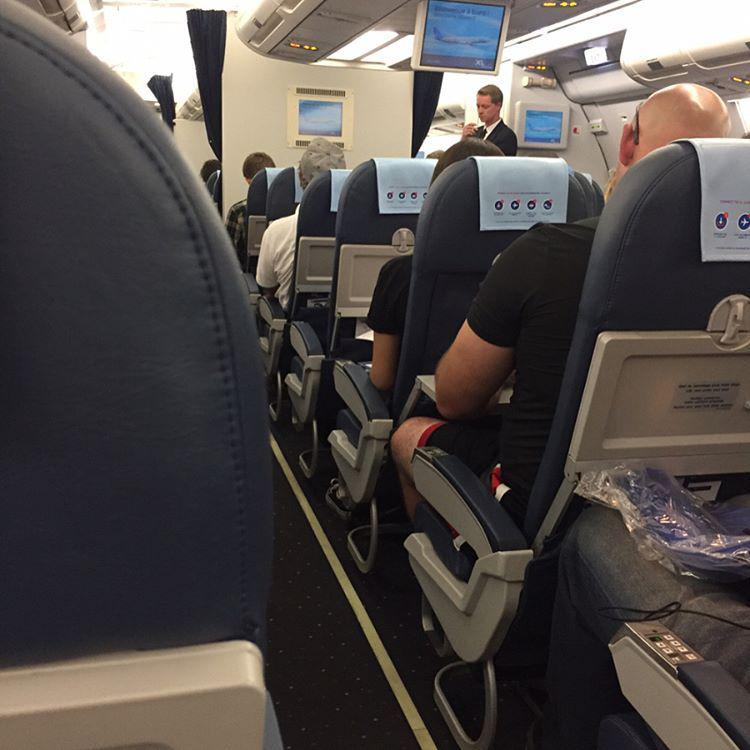
\includegraphics[width=0.5\linewidth]{Images/scared.jpg}
        \caption{``Planes might just be the most frightening thing ever." \textbf{scared}}
    \end{subfigure}
    \begin{subfigure}{.5\textwidth}
        \centering
        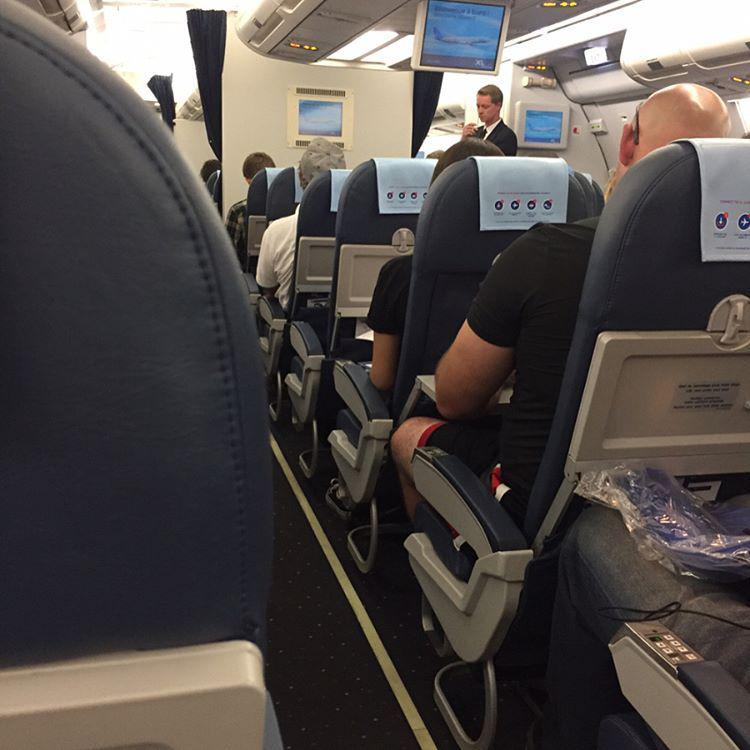
\includegraphics[width=0.5\linewidth]{Images/scared.jpg}
        \caption{``I hate it when people are taking too much space on planes." \textbf{angry}}
    \end{subfigure}
    \caption{Different meanings with different captions.}
    \label{ambiguous}
\end{figure}

Exploiting both visual and textual information is therefore key to understand the user's emotional state. Deep Sentiment is the name of the deep neural network incorporating visual recognition and text analysis.

\subsection{Architecture}
Deep Sentiment builds on the models we have seen before as shown in Figure \ref{deep-sentiment}:

\begin{figure}[H]
    \centering
    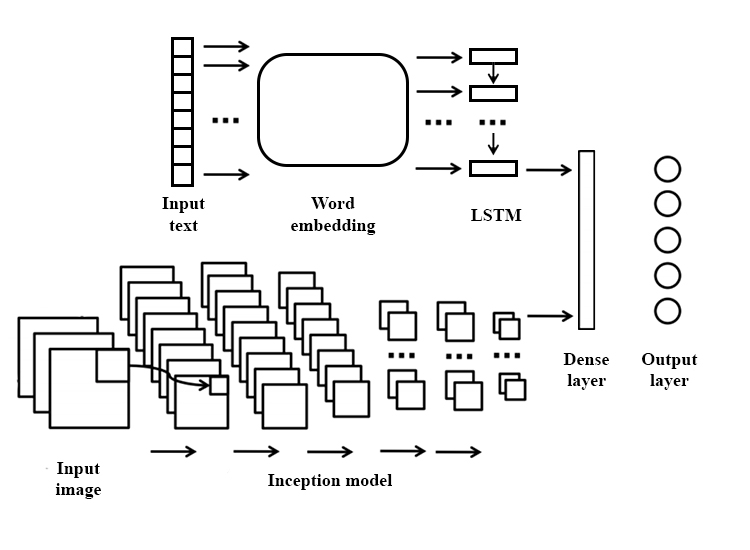
\includegraphics[width=0.6\textwidth]{Images/deep-sentiment-structure.jpg}
    \caption{The Deep Sentiment structure. On the one hand, the input image, resized to (224,224,3) is fed into the Inception network and outputs a vector of size 256. On the other hand, the text is projected into a high-dimensional space that subsequently goes through an LSTM layer with 1024 units. The two modalities are then concatenated and fed into a fully connected layer. The final softmax output layer give the probability distribution of the emotional state of the user.}
    \label{deep-sentiment}
\end{figure}

\section{Results}
Deep Sentiment was trained with the same configuration as before and figure \ref{train-validation} shows a comparison of the accuracy curves of the different models:

[Would like to use different learning rates for image and text. Also try bayesian hyperparameters optimisation]

\begin{figure}[H]
    \begin{subfigure}[t]{.5\textwidth}
        \vskip 0pt %Necessary to align on image and not caption
        \centering
        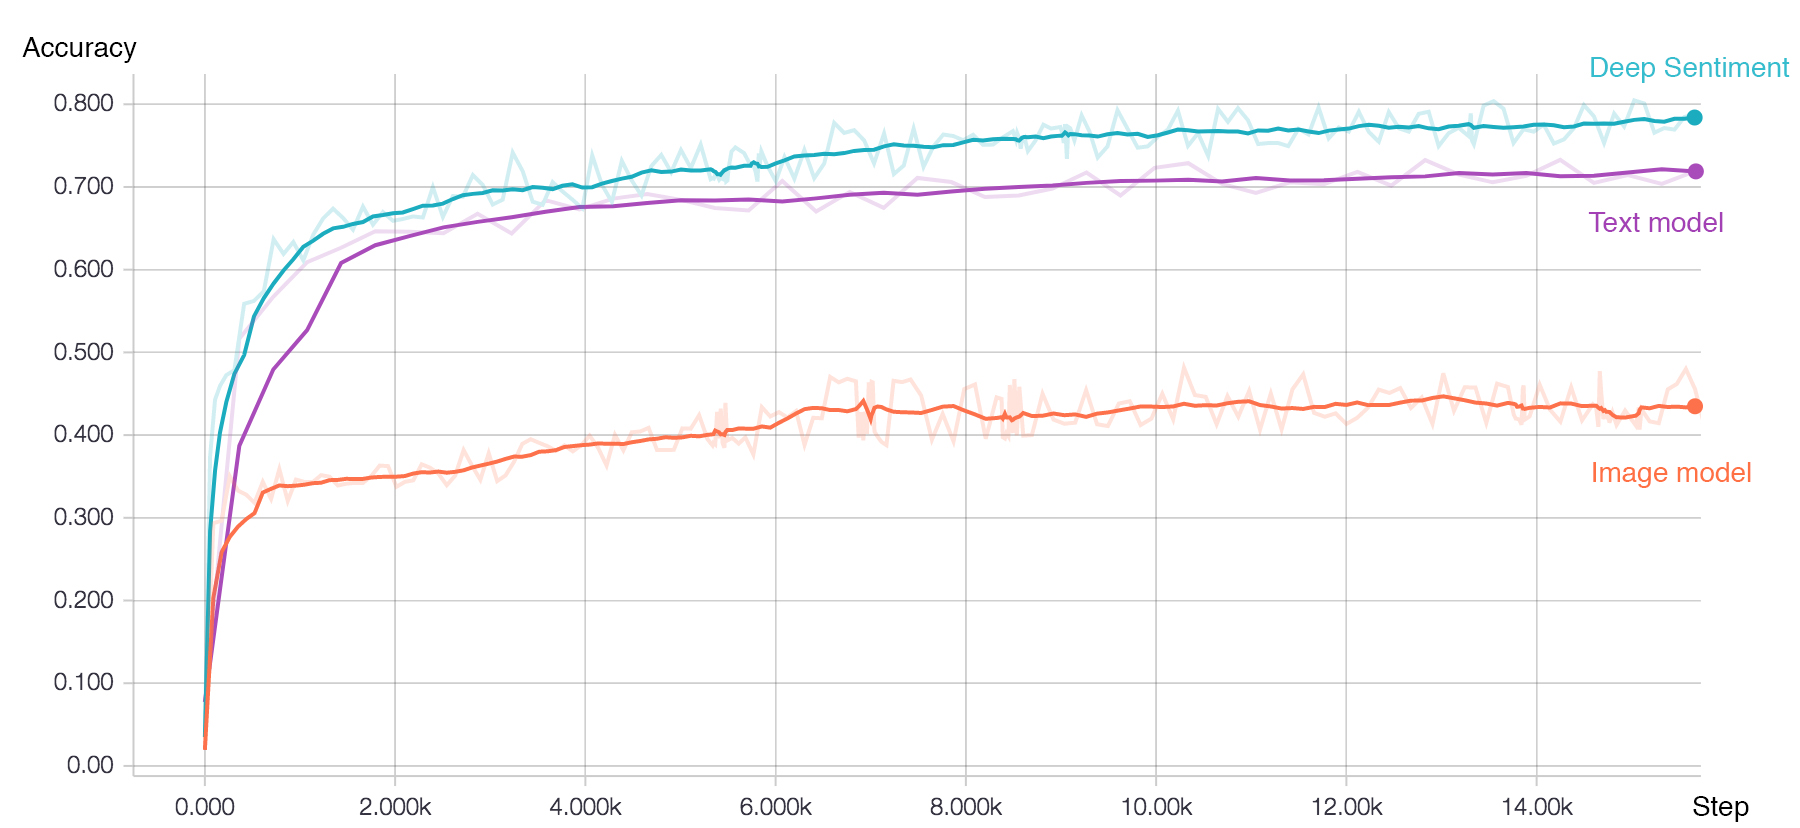
\includegraphics[width=\linewidth]{Images/train.jpg}
        \caption{Train curve}
   \end{subfigure}
   \begin{subfigure}[t]{.5\textwidth}
       \vskip 0pt
       \centering
       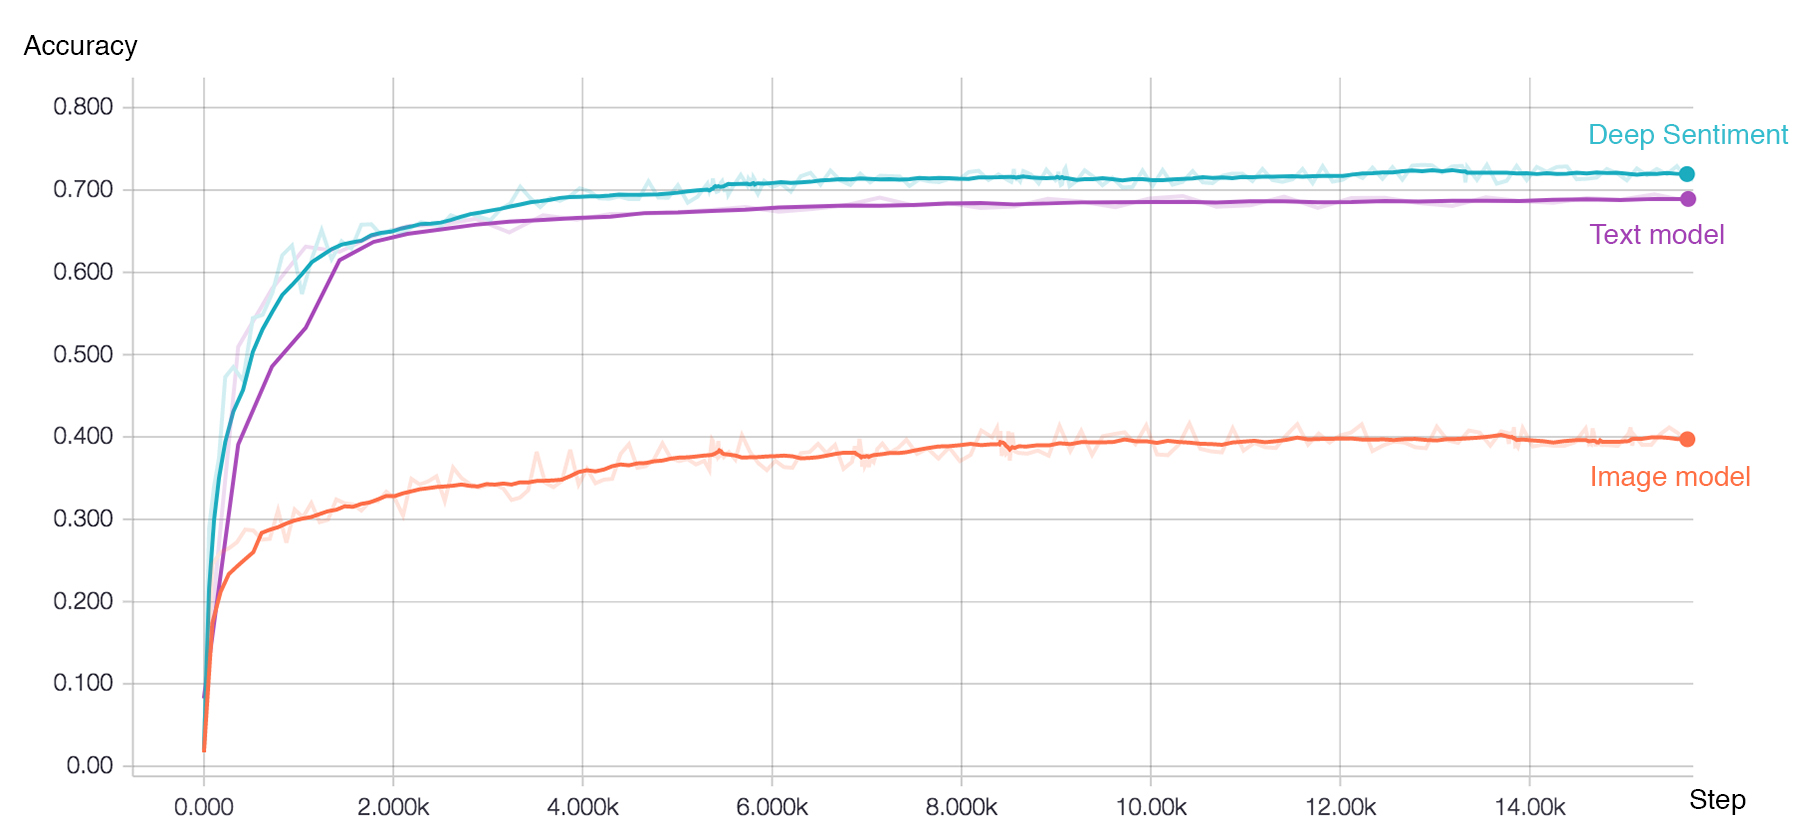
\includegraphics[width=\linewidth]{Images/validation.jpg}
       \caption{Validation curve}
    \end{subfigure}
    \caption{Accuracy curves}
    \label{train-validation}
\end{figure}

This model combining text and image outperforms the algorithms only using those elements separately with 80\% train accuracy and 72\% validation accuracy. This shows that just like a human being, a neural network needs both visual and textual information to determine the emotion conveyed by a post. The synergy between visual recognition and natural language processing is impressive as shown in the comparison table \ref{all-results}.

[Compute saliency maps on image and text as a sanity check: the network is looking at relevant words and objects to predict emotions]

\begin{table}[H]
\caption{Comparison of models}
\begin{center}
    \begin{tabular}{ l | c | c | c}
    & \textbf{Loss} & \textbf{Train} & \textbf{Validation} \\
    & & \textbf{accuracy} & \textbf{accuracy} \\ \hline
    \textbf{Random guessing} & - & 11\% & 11\% \\ \hline
    \textbf{Inception fine-tuned}  & 1.80 & 43\% & 36\% \\ \hline
    \textbf{LSTM model} & 0.81 & 72\% & 69\% \\ \hline
    \textbf{Deep Sentiment} & \textbf{0.75} & \textbf{80\%} & \textbf{72\%} \\
    \end{tabular}
\end{center} 
\label{all-results}
\end{table}

Given an image $\mathcal{I}$ and text $\mathcal{T}$, Deep Sentiment computes the conditional probabilities of the classes given the input image and input text. The outputs $(y_i)_{i=1}^n \in [0,1]^{16}$ are sampled from the distribution $Y| I, T$ where $I$ is the distribution of images $\mathcal{I}$ and $T$ the distribution of text $\mathcal{T}$. Using $(y_i)_{i=1}^n$, the empirical correlation matrix of the different emotions can be computed. Correlations is a measure of similarity and as such the correlations can be used as a distance matrix to obtain ahierarchical clustering of the emotions as shown in figure \ref{dendrogram}.

\begin{figure}[H]
    \centering
    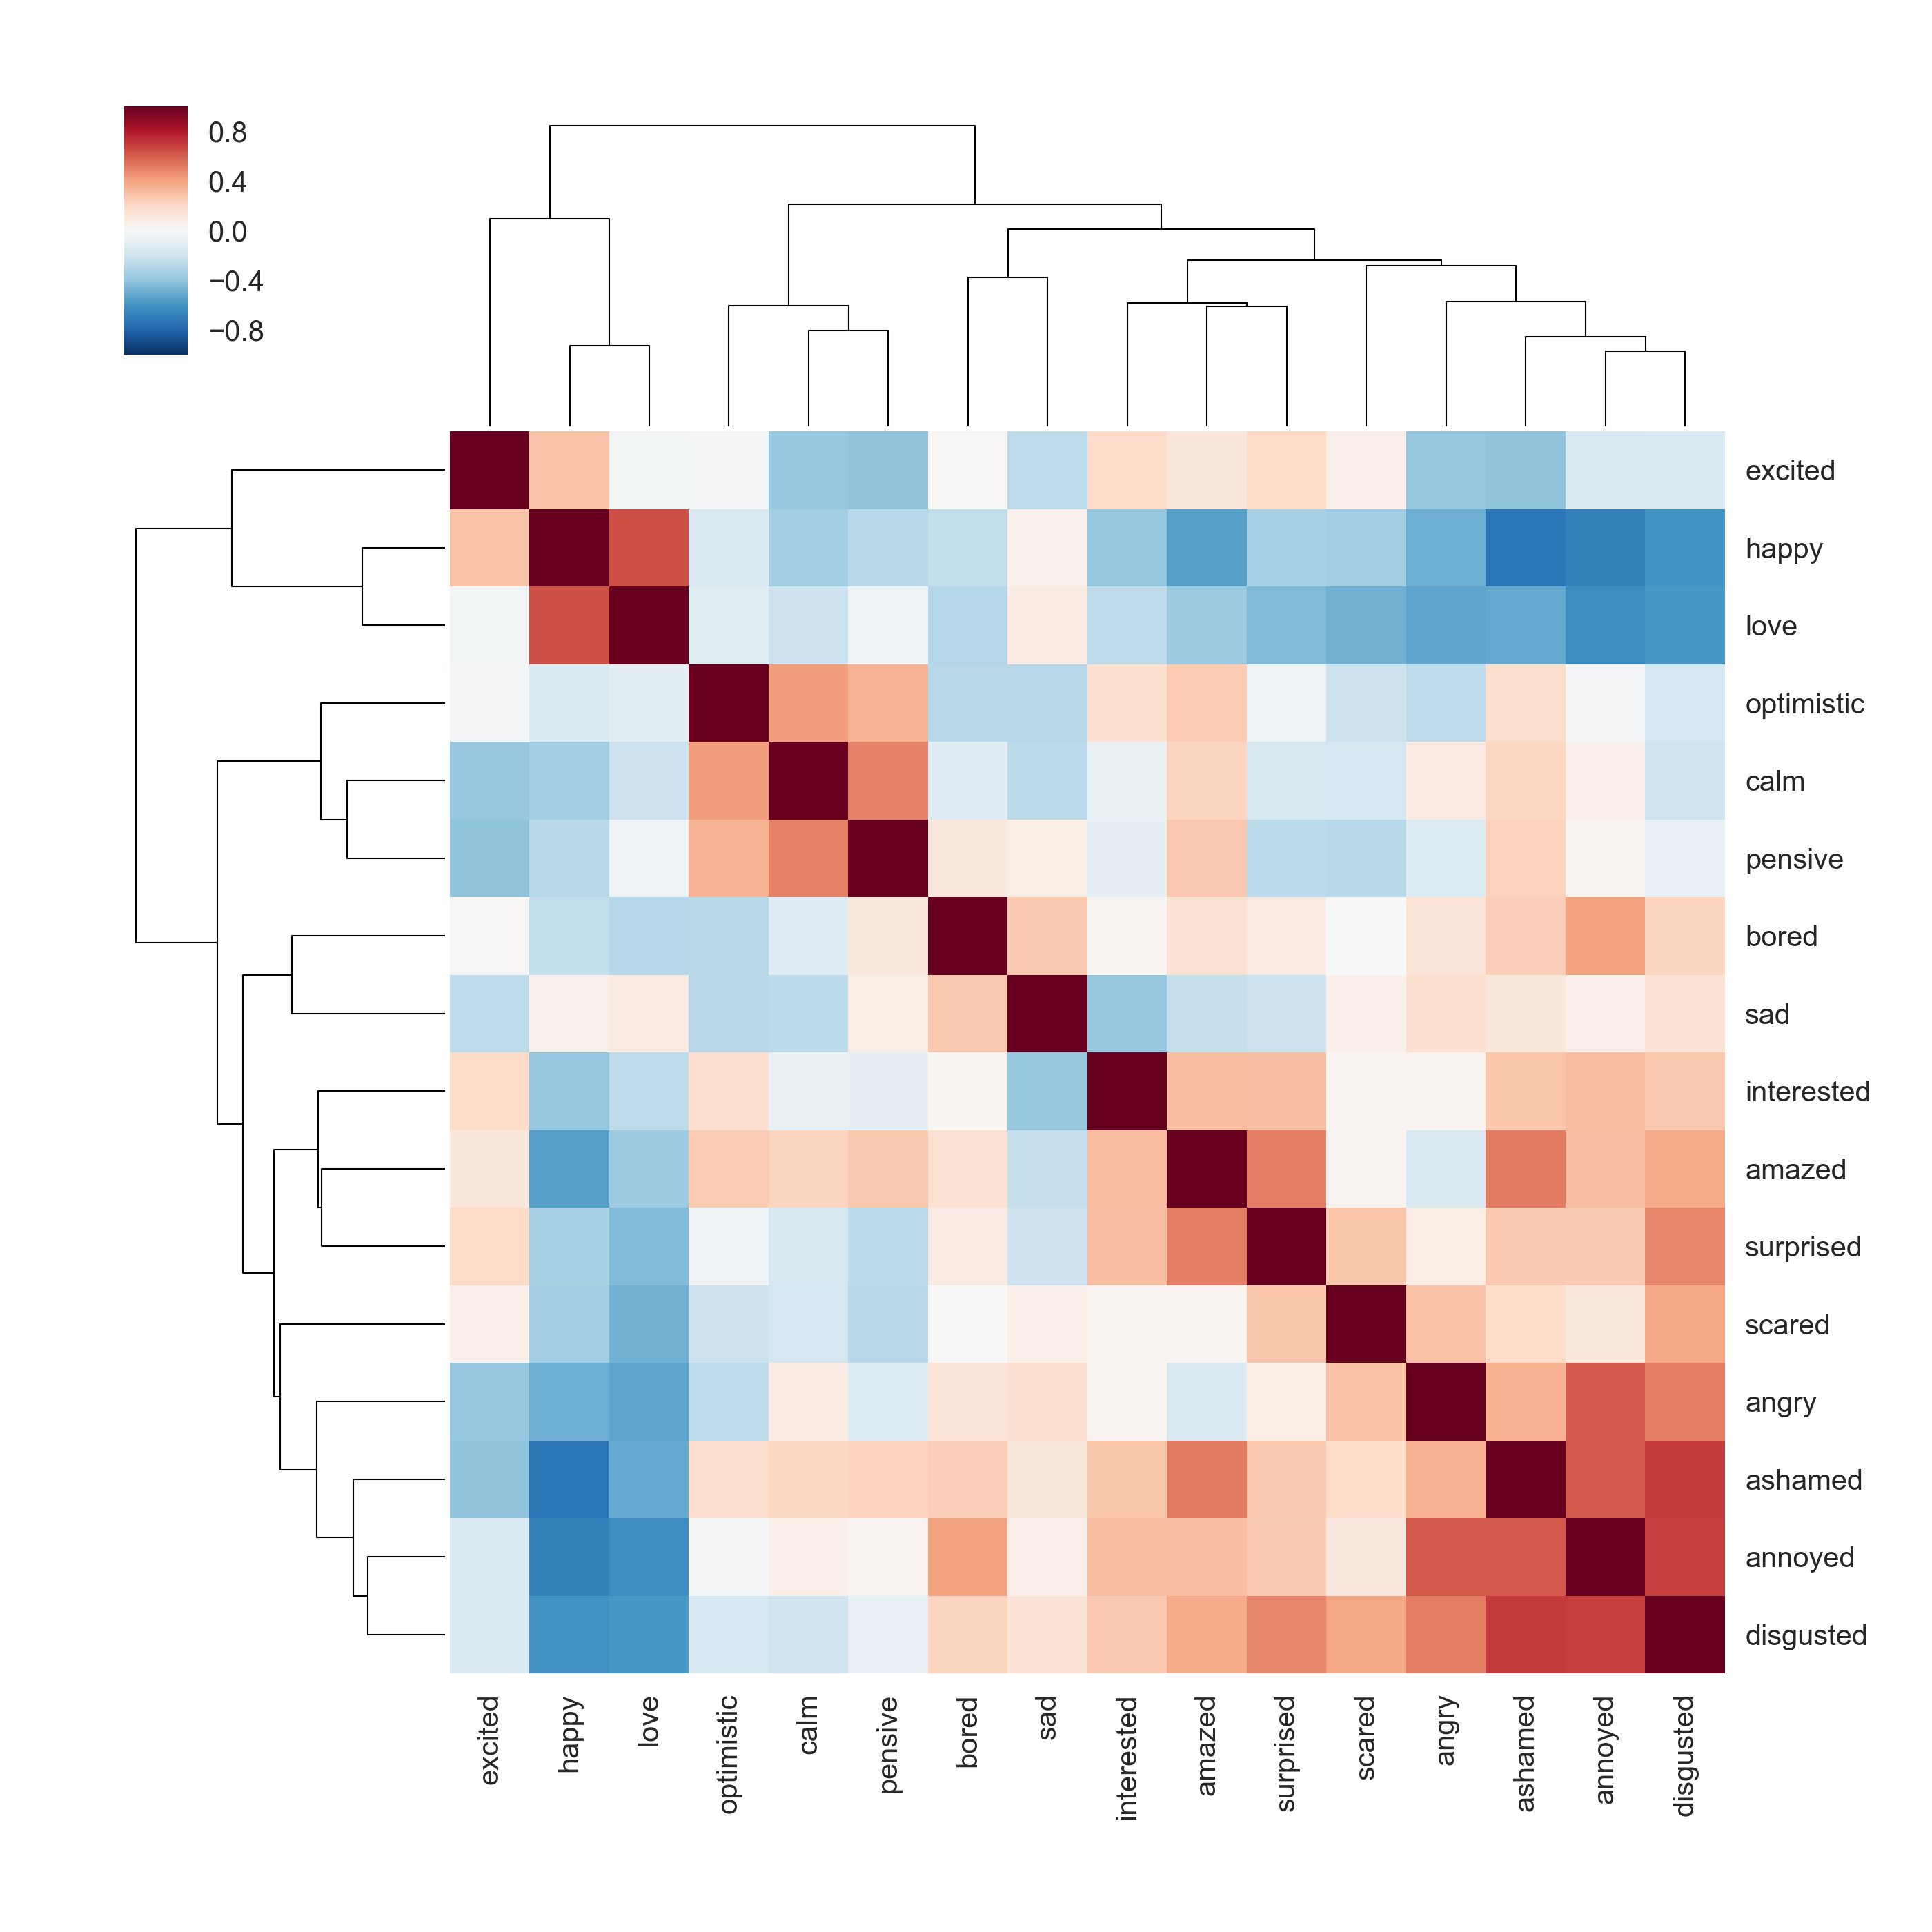
\includegraphics[width=0.8\textwidth]{Images/dendrogram.jpg}
    \caption{Hierarchically-clustered heatmap of the emotion correlation matrix}
    \label{dendrogram}
\end{figure}

There is a clear distinction between emotions that can be deemed as \textbf{positive} such as: `excited', `happy', `love', `optimistic' and \textbf{negative}: `scared', `angry', `ashamed', `annoyed', `disgusted'. In between lies ambivalent feelings such as `surprised' or `amazed'. The hierarchical clustering formed relevant clusters such as `happy' and `love', `calm' and `pensive' or `amazed' and `surprised'.

[Just computed this matrix, obviously need to analyse it more thoroughly.]
[Would like to know the proportion of misclassified examples that fall within emotions that are clustered in a distance of 1, then distance of 2 etc. Hopefully most mistakes come from clusters of distance 1.]



\subsubsection*{Acknowledgments}

\bibliography{iclr2018_conference}
\bibliographystyle{iclr2018_conference}

\end{document}
